\documentclass[aspectratio=169, xcolor=table]{beamer}
\usetheme{default}

% --- Packages ---
\usepackage{graphicx}
\usepackage{amsmath,amssymb}
\usepackage{booktabs}
\usepackage{tikz}
\usepackage{array}
\usepackage{multirow}
\usepackage{ragged2e}
\usepackage{animate}

\usetikzlibrary{shapes.geometric, arrows.meta, positioning, calc, fit, backgrounds, decorations.pathreplacing}

% --- Beamer Settings ---
\setbeamertemplate{navigation symbols}{}
\setbeamertemplate{footline}{%
  \hfill%
  \usebeamercolor[fg]{page number in head/foot}%
  \usebeamerfont{page number in head/foot}%
  \insertframenumber\,/\,\inserttotalframenumber%
  \kern1em\vskip1em%
}
\setbeamersize{text margin left=0.55cm, text margin right=0.55cm}

% --- Colors ---
\definecolor{highlightblue}{HTML}{0055A8}
\definecolor{highlightred}{HTML}{E37222}
\definecolor{darkgray}{HTML}{333333}
\definecolor{lightbluefill}{HTML}{EAF2FB}
\definecolor{lightredfill}{HTML}{FBEDE5}
\definecolor{lightgrayfill}{HTML}{F5F5F5}
\definecolor{lightgreenfill}{HTML}{EDF7ED}
\definecolor{hazardred}{HTML}{FF4444}
\definecolor{statenormal}{HTML}{4A90D9}
\definecolor{statequeuing}{HTML}{F5A623}
\definecolor{stateimpacted}{HTML}{D0021B}
\definecolor{statearrival}{HTML}{7ED321}
\definecolor{statesurvival}{HTML}{50C878}
\definecolor{statecasualty}{HTML}{8B0000}

\newcommand{\keyterm}[1]{\textbf{\textcolor{highlightblue}{#1}}}
\newcommand{\source}[1]{\par\vspace{-0.15em}{\raggedleft\fontsize{5.4}{6.0}\selectfont\textcolor{gray}{#1}\par}}
\newcommand{\parambox}[2]{\textcolor{highlightblue}{\textbf{#1}} {\scriptsize--- #2}}

% --- Style ---
\setbeamercolor{title}{fg=highlightblue}
\setbeamercolor{frametitle}{fg=highlightblue}
\setbeamerfont{frametitle}{series=\bfseries,size=\large}
\setbeamerfont{title}{series=\bfseries,size=\Large}
\setbeamercolor{block title}{bg=highlightblue!10, fg=darkgray}
\setbeamercolor{block body}{bg=highlightblue!3, fg=darkgray}
\setbeamercolor{alertblock title}{bg=highlightred!12, fg=darkgray}
\setbeamercolor{alertblock body}{bg=highlightred!4, fg=darkgray}
\setbeamercolor{item}{fg=highlightblue}
\setbeamertemplate{itemize item}{\color{highlightblue}$\blacktriangleright$}
\setbeamertemplate{itemize subitem}{\color{highlightblue}$\bullet$}
\setbeamertemplate{blocks}[rounded][shadow=false]

% --- TikZ styles ---
\tikzset{
  statebox/.style={rounded corners=4pt, minimum width=1.8cm, minimum height=0.85cm,
                   draw=black, thick, text=white, font=\small\bfseries, align=center},
  transarrow/.style={-{Stealth[length=5pt]}, thick, darkgray},
  panelbox/.style={draw=darkgray, rounded corners=6pt, thick, inner sep=6pt},
  flowbox/.style={rounded corners=3pt, minimum width=2.8cm, minimum height=0.6cm,
                  draw=black, thick, font=\scriptsize, align=center},
  flowdiamond/.style={diamond, minimum width=2.2cm, minimum height=1.0cm,
                      draw=black, thick, font=\scriptsize, align=center, inner sep=1pt},
}

% --- Meta ---
\title{Reproducing and Extending\\ a Multi-Agent Evacuation Simulation}
\subtitle{Final Project --- Shi, Lee, Yang (IEEE CASE 2024)}
\author{Dalal Alboloushi \quad \& \quad Jeongwon Bae}
\institute{IE 522 --- Simulation \\ Penn State University}
\date{Spring 2026 --- Final Presentation}

\begin{document}

% ============================================================
% SLIDE 1: TITLE
% ============================================================
\begin{frame}[plain]
  \titlepage
\end{frame}

% ============================================================
% SLIDE 2: Problem & Model recap (compressed from 1차)
% ============================================================
\begin{frame}[t,shrink=10]{Recap: Problem \& Three-Component Model}
\footnotesize

\begin{columns}[T,onlytextwidth]
\column{0.45\textwidth}
\textbf{Problem:} hazard strikes a community; thousands evacuate simultaneously.\\
Needed: agent-based sim capturing individual decisions + emergent congestion + panic.

\vspace{0.6em}
\begin{alertblock}{}
\scriptsize
Traditional process-flow models cannot capture emergent crowd dynamics.
$\Rightarrow$ \textbf{Multi-agent simulation} on a spatial network.
\end{alertblock}

\column{0.55\textwidth}
\vspace{-0.5em}
\begin{center}
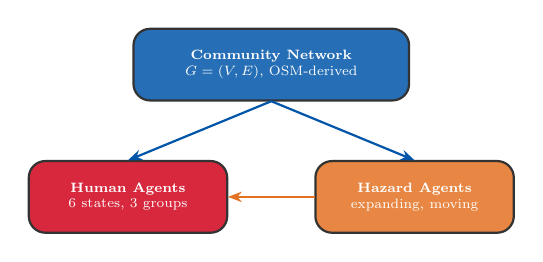
\begin{tikzpicture}[>=Stealth, font=\scriptsize, scale=0.70, transform shape]
  \node[panelbox, fill=highlightblue!85, text=white, minimum width=5cm, minimum height=1.3cm, align=center] (net) at (0, 2.2)
    {\textbf{Community Network}\\ {\scriptsize $G=(V,E)$, OSM-derived}};
  \node[panelbox, fill=stateimpacted!85, text=white, minimum width=3.6cm, minimum height=1.3cm, align=center] (human) at (-2.6, -0.2)
    {\textbf{Human Agents}\\ {\scriptsize 6 states, 3 groups}};
  \node[panelbox, fill=highlightred!85, text=white, minimum width=3.6cm, minimum height=1.3cm, align=center] (hazard) at (2.6, -0.2)
    {\textbf{Hazard Agents}\\ {\scriptsize expanding, moving}};
  \draw[transarrow, highlightblue] (net.south) -- (human.north);
  \draw[transarrow, highlightblue] (net.south) -- (hazard.north);
  \draw[transarrow, highlightred] (hazard.west) -- (human.east);
\end{tikzpicture}
\end{center}
\end{columns}
\source{Shi et al.\ (2024) --- presented in the midterm}
\end{frame}

% ============================================================
% SLIDE 3: Agents & Algorithms recap
% ============================================================
\begin{frame}[t,shrink=10]{Recap: Agents \& Algorithms 1--2}
\footnotesize

\begin{columns}[T,onlytextwidth]
\column{0.46\textwidth}
\textbf{Human states (6)} --- Normal, Queuing, Impacted, Arrival, Survival, Casualty.
Panic is \keyterm{irreversible}; impacted agents reroute to nearest shelter.

\vspace{0.4em}
\textbf{Hazards} --- circular impact zone, expanding and moving over time, with a lifespan.

\column{0.52\textwidth}
\begin{block}{\scriptsize Algorithm 2 --- Human$\leftrightarrow$Hazard (every step)}
\scriptsize
\begin{enumerate}\itemsep0.1em
  \item If agent inside hazard \& first impact $\to$ IMPACTED + reroute to shelter
  \item Casualty check (higher prob near center)
  \item Panic check (irreversible, $\varepsilon_p$ times group rate)
\end{enumerate}
\end{block}

\begin{block}{\scriptsize Algorithm 1 --- Human$\leftrightarrow$Network (every step)}
\scriptsize
\begin{enumerate}\itemsep0.1em
  \item If on edge $\to$ check edge congestion: queue or continue
  \item If at node $\to$ check node congestion: queue, reroute, random (panic), or advance
\end{enumerate}
\end{block}
\end{columns}
\source{Shi et al.\ (2024), Section III --- presented in the midterm}
\end{frame}

% ============================================================
% SLIDE 4: Reproduction scope
% ============================================================
\begin{frame}[t]{What we reproduced \& extended}
\footnotesize

\begin{columns}[T,onlytextwidth]
\column{0.48\textwidth}
\begin{block}{\small Paper reproduction targets}
\scriptsize
\begin{itemize}\itemsep0.2em
  \item \textbf{Phase 1} --- Table V, Fig.\ 3--4:\\
        networks for \textbf{5 communities}\\
        (PSU-UP, UVA-C, VT-B, RA-PA, KOP-PA)
  \item \textbf{Phase 2a} --- Fig.\ 5:\\
        $RI$ vs $P_{\max} \times H_{\max}$\\
        (9 configs, $\varepsilon_p = 10\%$)
  \item \textbf{Phase 2b} --- Fig.\ 6:\\
        $RS / RC / RL$ vs $\varepsilon_p$\\
        (5 paper points)
\end{itemize}
\end{block}

\column{0.48\textwidth}
\begin{alertblock}{\small Our extensions (beyond the paper)}
\scriptsize
\begin{itemize}\itemsep0.2em
  \item \textbf{Ext.\ \textcircled{\scriptsize 1}} Pmax \textbf{2K $\to$ 97K}\\
        (paper tested 2K--8K) --- breakpoint
  \item \textbf{Ext.\ \textcircled{\scriptsize 2}} Hmax \textbf{5 $\to$ 30}\\
        (paper tested 5--15) --- saturation
  \item \textbf{Ext.\ \textcircled{\scriptsize 3}} $\varepsilon_p$ \textbf{finer grid}\\
        (9 points vs paper's 5)
\end{itemize}
\end{alertblock}
\vspace{0.3em}
{\scriptsize 10 seeds per config; mean $\pm$ SD reported throughout.}
\end{columns}
\end{frame}

\end{document}
